\subsubsection{String-Patching (Win32)}

Man kann die Zeichenkette ''hello, world'' in der ausführbaren Datei mit Hiew finden:

\begin{figure}[H]
\centering
\myincludegraphics{patterns/01_helloworld/hola_edit1.png}
\caption{Hiew}
\label{}
\end{figure}

Man kann jetzt versuchen die Meldung ins Spanische zu übersetzen:

\begin{figure}[H]
\centering
\myincludegraphics{patterns/01_helloworld/hola_edit2.png}
\caption{Hiew}
\label{}
\end{figure}

Die spanische Version ist ein Byte kürzer als die englische, als muss am Ende ein 0x0A-Byte (\TT{\textbackslash{}n}) und ein Null-Byte eingefügt werden.

Es funktioniert.

Was wenn eine längere Nachricht eingefügt werden soll?
Hinter dem originalen englischen Text befinden sich einige Nullbytes.
Es ist schwierig zu sagen, ob diese überschrieben werden dürfen: es ist möglich, dass die zum Beispiel in dem \ac{CRT}-Code genutz werden. Vielleicht aber auch nicht.
Wie dem auch sei: diese Daten sollten nur überschrieben werden, wenn wirklich klar ist was man tut.

\subsubsection{String-Patching (Linux x64)}

\myindex{\radare}
Nachfolgend wird der Patch einer ausführbaren Datei unter einem 64 Bit-Linux mit \radare{} gezeigt:

\lstinputlisting[caption=\radare{} session]{patterns/01_helloworld/radare.lst}

Was hier passiert ist folgendes: suchen von \q{hello} mit dem \TT{/}-Kommando,
dann Setzen des \emph{cursor} (oder \emph{seek} im \radare{}-Wording) an diese Adresse.
Um sicher zu gehen, dass die richtige Stelle gesetzt ist, kann mit \TT{px} der Datenblock ausgegeben werden.
\TT{oo+} versetzt \radare{} in den \emph{Lese-Schreibe}-Modus.
\TT{w} schreibt einen ASCII string an die aktuelle Adresse.
Hinweis: \TT{\textbackslash{}00} am Ende ist das Null-Byte.
\TT{q} beendet \radare{}.

% TBT
%\subsubsection{This is a real story of software cracking}
%\label{\SoftwareCracking}
%
%An image processing software, when not registered, added watermarks,
%like ``This image was processed by evaluation version of [software name]'', across a picture.
%We tried at random: we found that string in the executable file and put spaces instead of it.
%Watermarks disappeared.
%Technically speaking, they continued to appear.
%\myindex{Qt}
%With the help of Qt functions, the watermark was still added to the resulting image.
%But adding spaces didn't alter the image itself...

\subsubsection{Software-\emph{Lokalisation} zu MS-DOS-Zeiten}

Der hier beschriebene Weg war in den 1980ern und  1990ern sehr vebreitet, um MS-DOS-Progamme in die russische Sprache zu übersetzen.
Russische Wörter und Sätze sind in der Regel etwas länger als ihre englischen Gegenstücke, was der Grund ist, dass
viele \emph{lokalisierte} Programme eine Menge seltsamer Akronyme und Abkürzungen haben.

\begin{figure}[H]
\centering
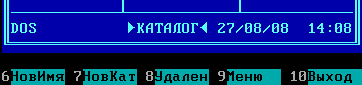
\includegraphics[width=0.5\textwidth]{patterns/01_helloworld/Norton_Commander_v5_51.png}
\caption{\DEph{}}
\end{figure}

Möglicherweise passierte dies in der Zeit auch in anderen Sprachen.
